
\section{Single cells analysis}
\label{chap:UnitsAnalysis}
The aim of the project is to understand the nature of interactions between Ventral Striatum (VS) and Ventral Tegmental Area (VTA). Loops and circuit effects make puzzling to understand the whole picture of the aforementioned interactions (figure\ref{fig:Brain}, left). To see how specific interactions are involved in the prediction coding is needed a cell-types classification of underlying units.\\
In this chapter we present the cell types classification provided by Max Scheller.
\begin{figure}
    \centering
    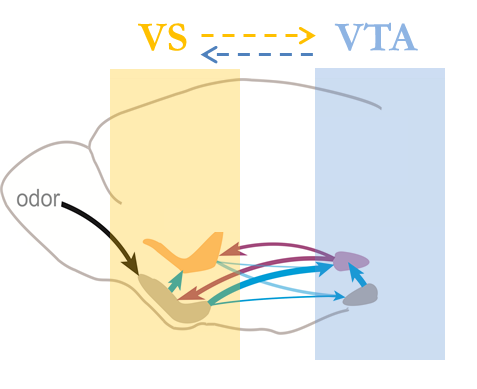
\includegraphics[width=0.45\textwidth]{BrainVSVTA.png}
    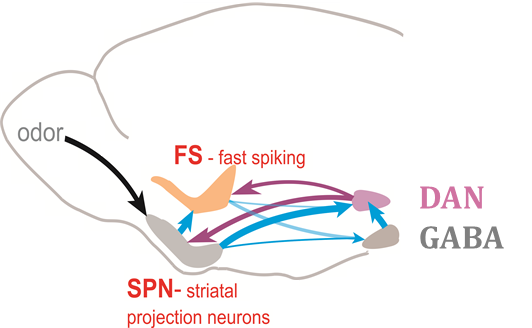
\includegraphics[width=0.45\textwidth]{Brain.png}
    \caption{Caption}
    \label{fig:Brain}
\end{figure}
The data-set included $803$ VS and pallidal units and $272$ VTA units in total, that were classified in sub-types. Specifically VS units were classified as either striatal projection neurons (SPNs), fast-spiking neurons (FSNs) or cholinergic interneurons(CINs), according to their firing pattern characteristics computed using only spikes during the inter-trials interval and after session. Units with a firing rate higher than $12 Hz$ were assigned as FSNs and all units with a firing rate below $2 Hz$ as SPNs. Units in the remaining range were designed as putative regular-firing CINs if the CV or their $ISI$ distribution was less than $1.2$ and ISIs less than $60 ms$ contributed no more than $20\%$ of all ISIs (\cite{Inokawa}). Finally the resting units were characterized as SPNs or FSNs if they ever were silent for more than $2 s$ (\cite{Graybiel}). Using this classification mean normalized autocorrelations and mean waveforms have canonical patterns.\\ The VS consists of the nucleus accumbens and the olfactory tubercle (OTu).
Considering the close anatomical relationship between OT and VP (\cite{Heimer1982}) and the statistics of cell types in the two regions (FSNs in Striatum represent only $<5\%$ of the population({\color{red}askfor paper to cite}), while pallidal units have higher firing rate ({\color{red}askfor paper to cite}), it can be assumed that the recorded FSNs are pallidal neurons.\\
VTA units were instead classified as dopaminergic neurons (DAN), gabaergic units (GABA), and glutamatergic neurons (GLU) according to their task related activity using a clustering approach adapted from (\cite{Uchida}). First, response were characterized for the relevant time spans ({\color{red}ask Max for the updated intervals}(CS+ from 0 to 0.5 and US from -0.5 to 0 and from 0 to 0.5), significant task related response were assessed with Friedman test, and only significant units ($p<0.05$) were included in the clustering classification.{\color{red}part of classification has to be included}
\begin{figure}
  \centering
    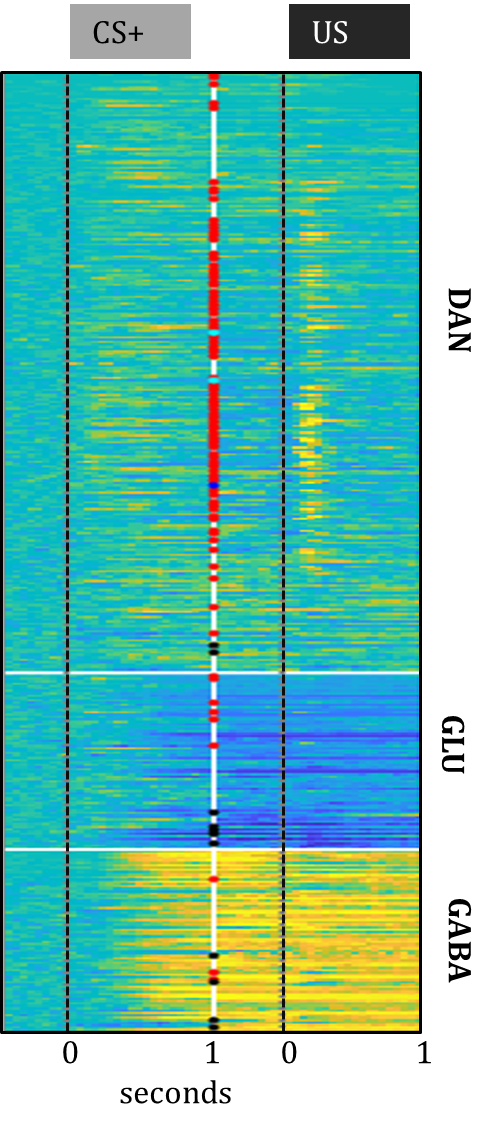
\includegraphics[scale=0.75]{figures/ClassificationUnits.png}
   \caption{Figure provided by Max Scheller. VTA classification according to units task related activity using a clustering approach adapted from (\cite{Uchida}). In this study we focused on dopaminergic and gabaergic units in assemblies. Dopaminergic units show a phasic response to the reward, whereas gabaergic units are tonically active neurons.}
    \label{fig:ClassificatonVTA}
\end{figure}
Considering the units recorded in paradigms used for the assembly analysis, the cell-types result to occur in VS and VTA as shown in figure\ref{fig:PieRegions}.
\begin{figure}
  \centering
    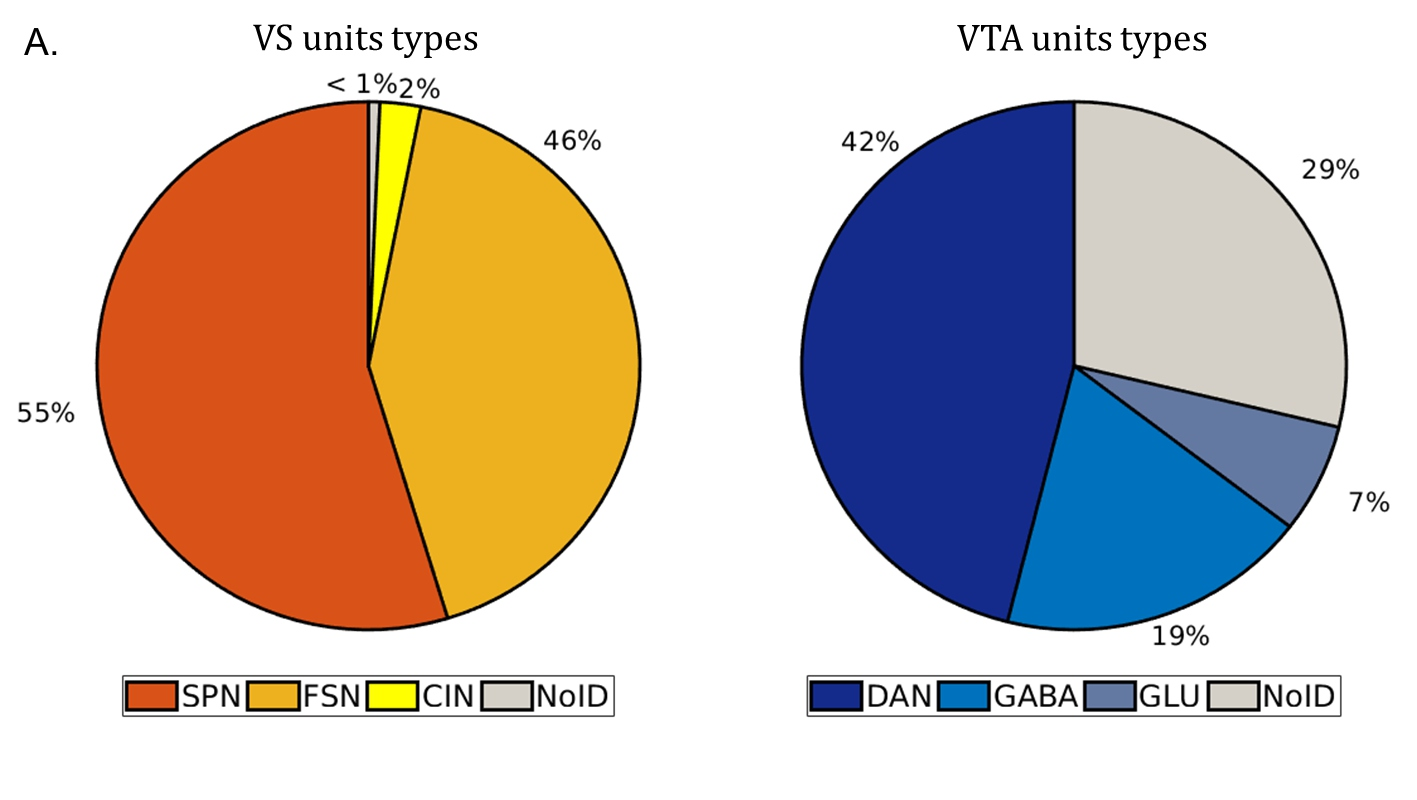
\includegraphics[scale=0.5]{figures/PieRegions1.pdf}
   \caption{Left: units types pie chart in Ventral Striatum. Right: units types pie chart in Ventral Tegmental Area}
    \label{fig:PieRegions}
\end{figure}

